\begin{figure}[!h]
\centering
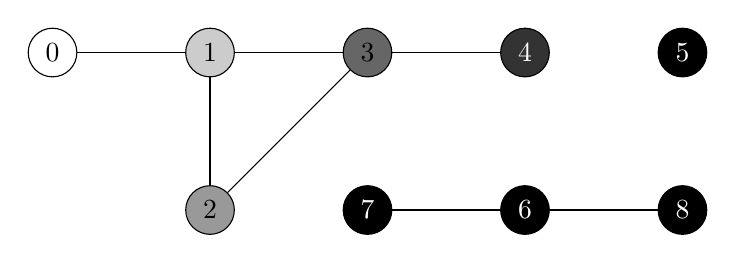
\begin{tikzpicture}[scale=1, label1/.style = {circle,fill=black!0,draw}, label2/.style = {circle,fill=black!20,draw}, label3/.style = {circle,fill=black!40,draw}, label4/.style = {circle,fill=black!60,draw}, label5/.style = {circle,fill=black!80,draw,text=white}, label6/.style = {circle,fill=black!100,draw, text=white}, edge/.style = {-,thin}]
% vertex
\node[label1] (n0) at (1,3)  {0};
\node[label2] (n1) at (3,3)  {1};
\node[label4] (n3) at (5,3)  {3};
\node[label5] (n4) at (7,3)  {4};
\node[label6] (n5) at (9,3)  {5};
\node[label3] (n2) at (3,1)  {2};
\node[label6] (n7) at (5,1)  {7};
\node[label6] (n6) at (7,1)  {6};
\node[label6] (n8) at (9,1)  {8};
%edges
\draw[edge] (n0) to (n1);
\draw[edge] (n1) to (n2);
\draw[edge] (n0) to (n1);
\draw[edge] (n1) to (n3);
\draw[edge] (n3) to (n4);
\draw[edge] (n3) to (n2);
\draw[edge] (n7) to (n6);
\draw[edge] (n6) to (n8);
\end{tikzpicture}
\caption{Ejemplo de búsqueda en profundidad}
Dado un grafo conexo no direccionado, se realiza la búsqueda en profundidad en $s=0$, obteniendo el siguiente recorrido $0 \rightarrow 1 \rightarrow 2 \rightarrow 3 \rightarrow 4$. \\Fuente: \cite{Halim2019}.
\label{ejemDfs}
\end{figure}